% 等边三角形 + 高 → 拆为两个 30-60-90
\documentclass[tikz,border=4pt]{standalone}
\usepackage{ctex}
\usepackage{amsmath}
\usetikzlibrary{decorations.markings}
\begin{document}
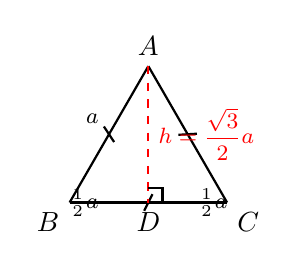
\begin{tikzpicture}[scale=1.0, thick,
  tick/.style={postaction={decorate, decoration={markings,
    mark=at position 0.5 with {\draw (-1.5pt,-3pt) -- (1.5pt,3pt);}}}}]
  \coordinate (A) at (0, {sqrt(3)});
  \coordinate (B) at (-1, 0);
  \coordinate (C) at ( 1, 0);
  \coordinate (D) at (0, 0);
  \draw[tick] (A) -- (B);
  \draw[tick] (A) -- (C);
  \draw[tick] (B) -- (C);
  \draw[red, dashed] (A) -- (D);
  \draw (0.18, 0) -- (0.18, 0.18) -- (0, 0.18);

  \node[above] at (A) {$A$};
  \node[below left] at (B) {$B$};
  \node[below right] at (C) {$C$};
  \node[below] at (D) {$D$};

  \node[left]  at (-0.5, 0) {\footnotesize $\tfrac{1}{2}a$};
  \node[right] at ( 0.5, 0) {\footnotesize $\tfrac{1}{2}a$};
  \node[right, red] at (0, {sqrt(3)/2}) {\footnotesize $h=\dfrac{\sqrt{3}}{2}a$};
  \node[above left] at (-0.5, {sqrt(3)/2}) {\footnotesize $a$};
\end{tikzpicture}
\end{document}
